\subsection{Radiation Portal Monitors}
%%%%%%%%%%%%%%%%%%%%%%%%%%%%%%%%%%%%%%%%%%%%%%%%%%%%%%%%%%%%%%%%%%%%%%%%%%%%%%%
\begin{frame}{U.S. Border Traffic}
\begin{columns}[onlytextwidth]
\begin{column}{0.45\textwidth}
  \begin{itemize}
  \item Every day 932,456 people cross into the U.S. \cite{cpb_typical_2012}
    \begin{itemize}
    	\item 259,191 by air
	\item 48,073 by sea
	\item 621,874 by land
    \end{itemize}
  \item 64,483 truck, rail and sea containers \cite{cpb_typical_2012}
 \item 253,821 privately-owned vehicles \cite{cpb_typical_2012}
  \end{itemize}
\end{column}
\begin{column}{0.45\textwidth}
  \begin{figure}[ht]
    \vspace*{-3cm}
		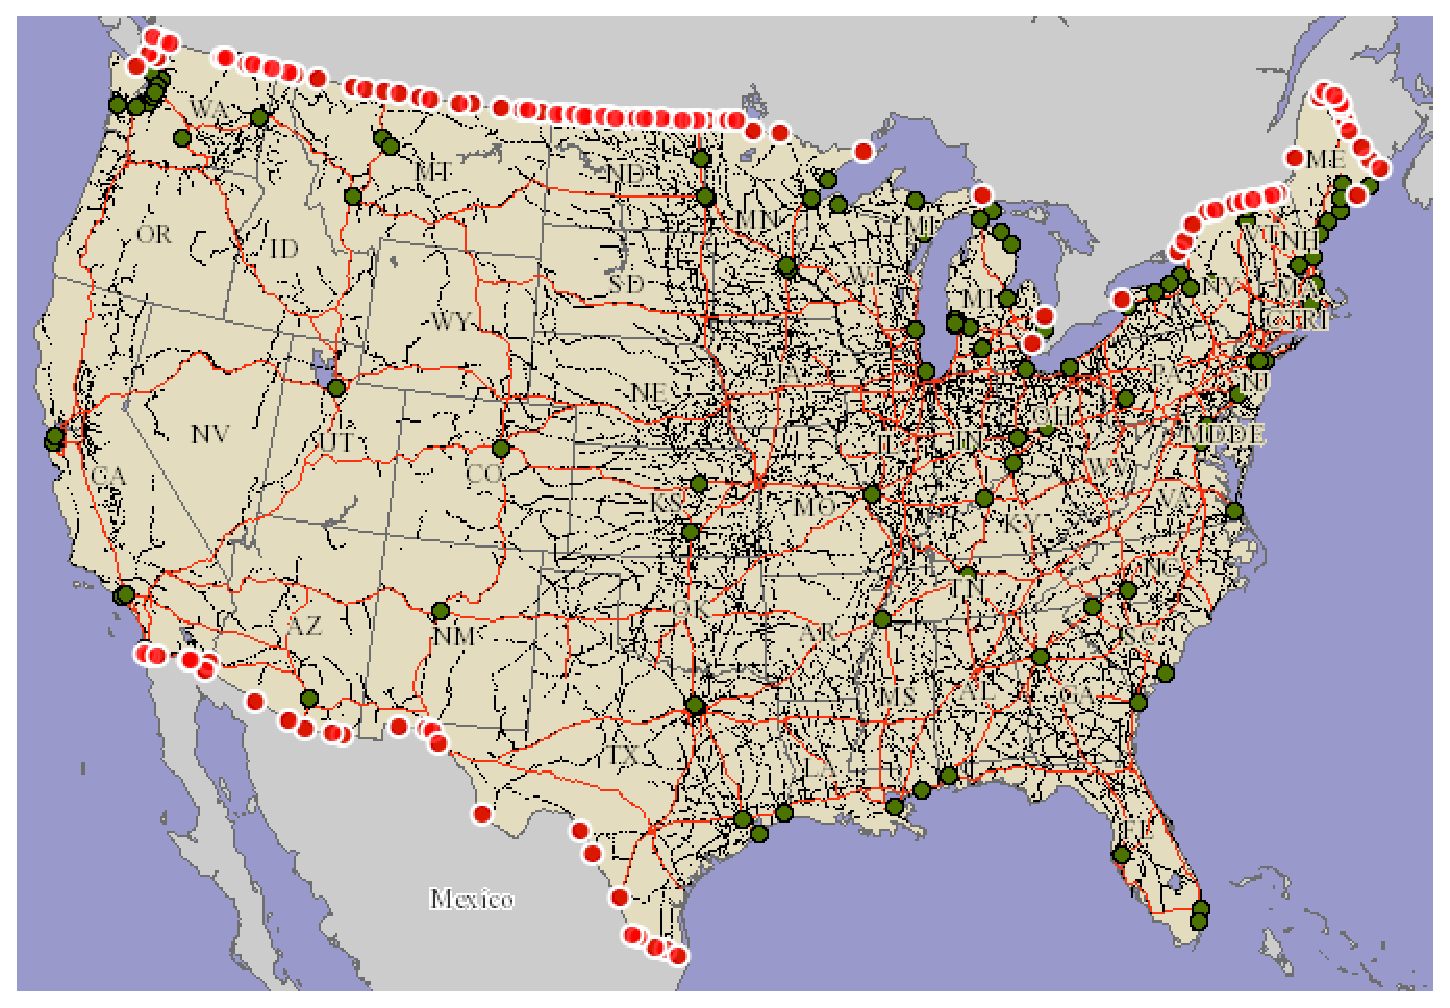
\includegraphics[width=\textwidth]{PortalEntryMap.eps}
  \end{figure}
\end{column}
\end{columns}
\end{frame}

%%%%%%%%%%%%%%%%%%%%%%%%%%%%%%%%%%%%%%%%%%%%%%%%%%%%%%%%%%%%%%%%%%%%%%%%%%%%%%%
\begin{frame}{Radiation Portal Monitors}
\begin{columns}[onlytextwidth]
	\begin{column}{0.45\textwidth}
  	\begin{itemize}
  		\item Radiation portal monitors (RPMs) are passive radiation detectors
  		\item {
  			 RPMs are currently   ${}^3$He based detectors
  			\center
    		${}^3He +n \to p +{}^3H$
    	}
  		\item Shortage of ${}^3$He, so alternatives are being explored
		  \item ${}^6Li + n \to {}^3H + \alpha$    
  		\end{itemize}
	\end{column}
	\begin{column}{0.5\textwidth}
		\begin{figure}
    \vspace*{-3cm}
      \centering
			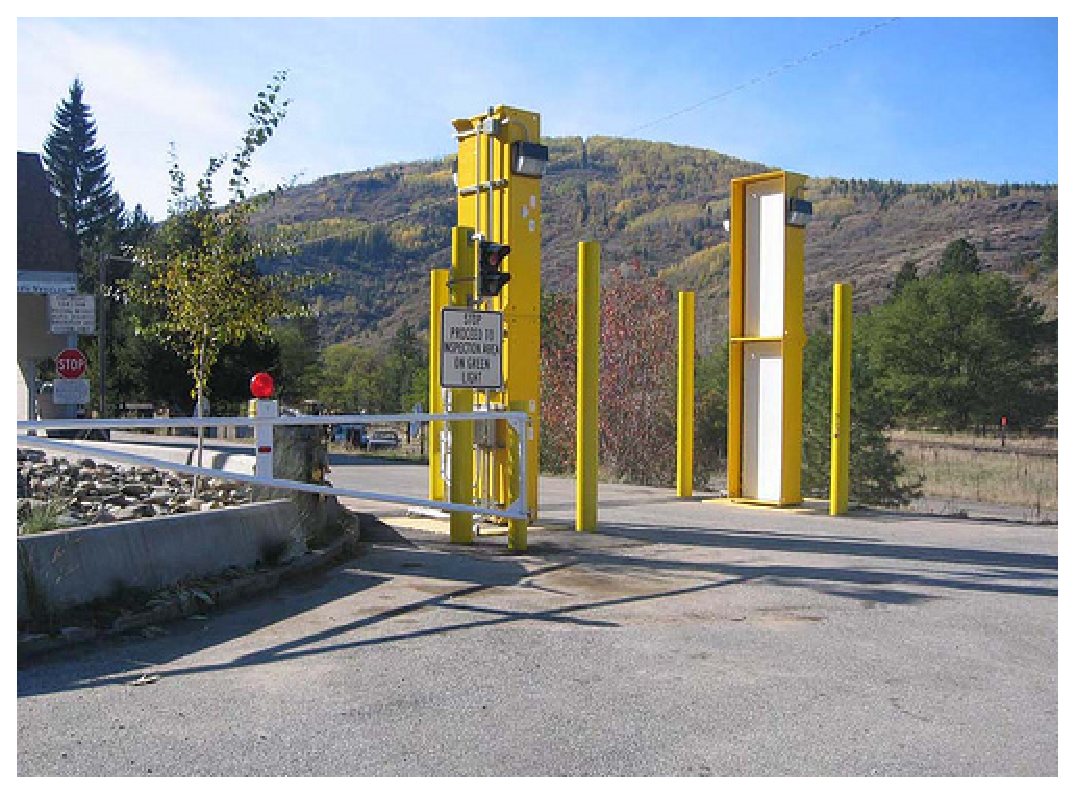
\includegraphics[width=\textwidth]{RPM8_Installed.eps}
    \end{figure}
	\end{column}
\end{columns}
\end{frame}
%%%%%%%%%%%%%%%%%%%%%%%%%%%%%%%%%%%%%%%%%%%%%%%%%%%%%%%%%%%%%%%%%%%%%%%%%%%%%%%

\subsection{Detector Requirements}
%%%%%%%%%%%%%%%%%%%%%%%%%%%%%%%%%%%%%%%%%%%%%%%%%%%%%%%%%%%%%%%%%%%%%%%%%%%%%%%
\begin{frame}{Detector Requirements}
DHS / DNDO (along with PNNL) has determined a set of objectives that replacement technologies should meet:
\begin{table}
	\small
	\begin{tabular}{ m{5cm} m{5cm} }
	Parameter & Specification \\
	\hline
	\hline
	Absolute neutron detection efficiency & 2.5 cps/ng of ${}^{252}Cf$ (in specified test configuration) \\
	Intrinsic gamma-neutron detection efficiency & $ \epsilon_{int,\gamma n}\leq 10^{-6}$ \\
	Gamma absolute rejection ratio for neutrons (GARRn) & $ 0.9 \leq \text{ GARRn }\leq$ 1.1 at 10 mR/h exposure \\
	Cost &  \$ 30,000 per system \\
	\hline
	\end{tabular}
\end{table}
\hyperlink{PNNLCriteria}{\beamerbutton{Detailed Criteria}}
\label{DHSCriteria}
\end{frame}

%%%%%%%%%%%%%%%%%%%%%%%%%%%%%%%%%%%%%%%%%%%%%%%%%%%%%%%%%%%%%%%%%%%%%%%%%%%%%%%
%                                                                             %
%                                PREVIOUS WORK                                %
%                                                                             %
%%%%%%%%%%%%%%%%%%%%%%%%%%%%%%%%%%%%%%%%%%%%%%%%%%%%%%%%%%%%%%%%%%%%%%%%%%%%%%%
\subsection{Previous Work}

%%%%%%%%%%%%%%%%%%%%%%%%%%%%%%%%%%%%%%%%%%%%%%%%%%%%%%%%%%%%%%%%%%%%%%%%%%%%%%%
\begin{frame}[fragile]{Replacement Technologies}
\begin{columns}[onlytextwidth]
\begin{column}{0.55\textwidth}
\begin{itemize}
	\small
	\item Boron Straw Tubes (Proportional Technology) \cite{kouzes_boron-lined_2012}
	\begin{itemize}
    %\tiny
		\item Count rate meets requirements
		\item Gamma rejection is estimated to be $4x10^{-9}$
		\item GARRn within desired range
	\end{itemize}
	\small
	\item LiF:ZnS coated Paddles (IAT) \cite{kouzes_lithium_2010}
	\begin{itemize}
    %\tiny
		\item Did not fulfill the neutron count rate
		\item Adequate gamma ray rejection
		\item Passed the GARRn
	\end{itemize}
\end{itemize}
\end{column}
\begin{column}{0.4\textwidth}
	\begin{figure}
    \centering
    \begin{subfigure}[b]{\textwidth}
      \centering
		  \includegraphics[height=0.25\textheight]{B10StrawFibers.eps}
      \caption{ ${}^{10}$B Straw Fibers}
      \label{fig:B10StrawFibers}
    \end{subfigure}

    \begin{subfigure}[b]{\textwidth}
      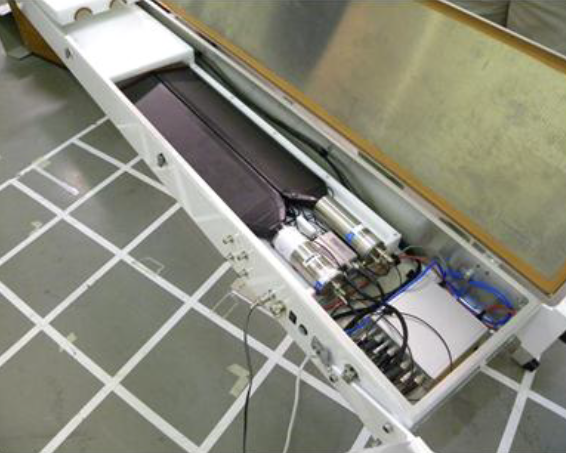
\includegraphics[height=0.25\textheight]{IATImage}
      \caption{${}^6$LiF:ZnS Paddle}
      \label{fig:LifZnSPaddle}
    \end{subfigure}
	\end{figure}
\end{column}
\end{columns}
\end{frame}
%%%%%%%%%%%%%%%%%%%%%%%%%%%%%%%%%%%%%%%%%%%%%%%%%%%%%%%%%%%%%%%%%%%%%%%%%%
%                                                                        %
%                            INTRODUCTION                                %
%                                                                        %
%%%%%%%%%%%%%%%%%%%%%%%%%%%%%%%%%%%%%%%%%%%%%%%%%%%%%%%%%%%%%%%%%%%%%%%%%%
\subsection{UT Fabricated Films}
%%%%%%%%%%%%%%%%%%%%%%%%%%%%%%%%%%%%%%%%%%%%%%%%%%%%%%%%%%%%%%%%%%%%%%%%%%
\begin{frame}{UT Fabricated Polymeric Detectors}
\label{PHDMain}
  \begin{itemize}
    \item Films are characterized on-site
    \item Gamma ray rejection achieved through a pulse height discriminator
  \end{itemize}
  \centering{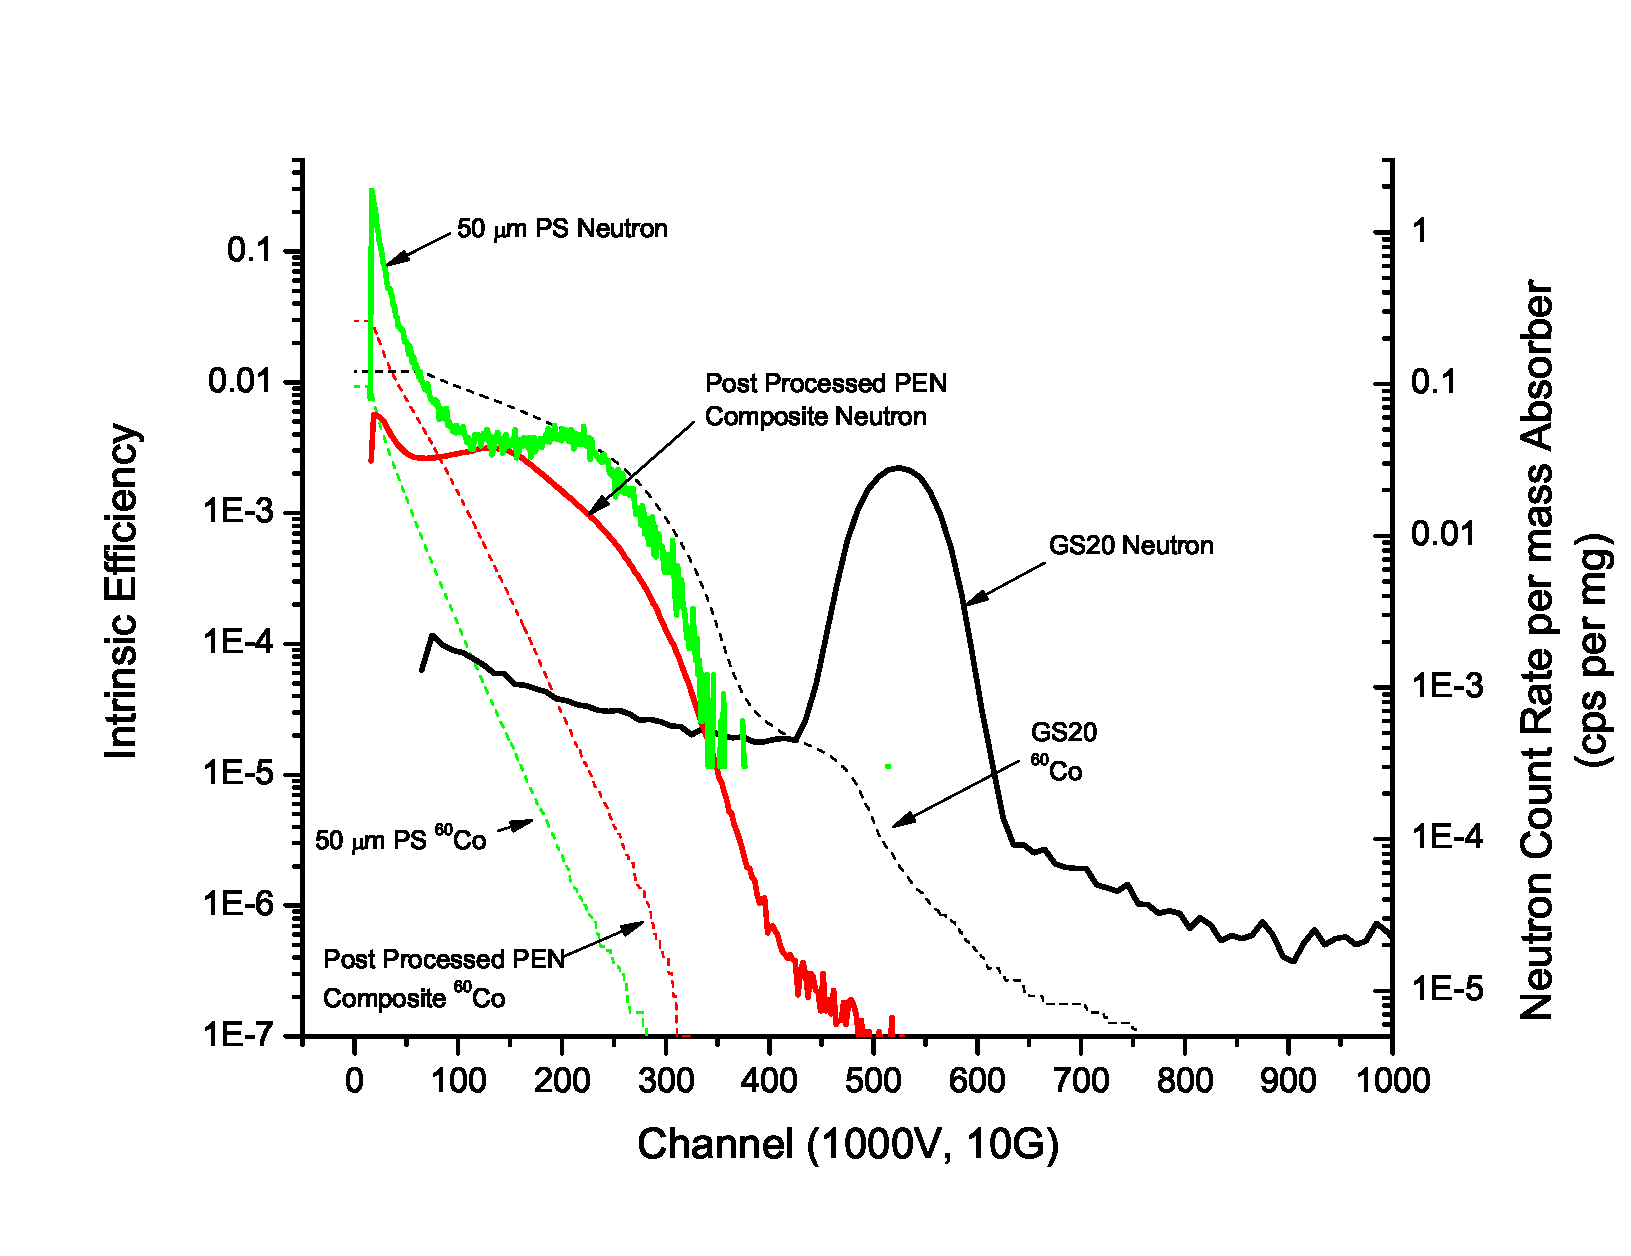
\includegraphics[height=0.6\textheight]{SC_UTDetectors_IntEff_CR}}

\hyperlink{MeasMethods}{\beamerbutton{Measurment Setups and Methods}}
\end{frame}
%%%%%%%%%%%%%%%%%%%%%%%%%%%%%%%%%%%%%%%%%%%%%%%%%%%%%%%%%%%%%%%%%%%%%%%%%%
